%% PNAStwoS.tex
%% Sample file to use for PNAS articles prepared in LaTeX
%% For two column PNAS articles
%% Version1: Apr 15, 2008
%% Version2: Oct 04, 2013

%% BASIC CLASS FILE
\documentclass{pnastwo}

%% ADDITIONAL OPTIONAL STYLE FILES Font specification

%\usepackage{pnastwoF}
\usepackage[sort&compress]{natbib}

%% OPTIONAL MACRO DEFINITIONS
\def\s{\sigma}
%%%%%%%%%%%%
%% For PNAS Only:
\url{}
\copyrightyear{}
\issuedate{Issue Date}
\volume{Volume}
\issuenumber{Issue Number}
%\setcounter{page}{} %Set page number here if desired
%%%%%%%%%%%%

\begin{document}

\title{Conflict and Strategy in Collective Computation}

\author{Eleanor Brush\affil{1}{Princeton University, Princeton, NJ, USA}\affil{2}{Wisconsin Institute for Discovery, University of Wisconsin, Madison, USA},
David Krakauer \affil{2}{}\affil{3}{Santa Fe Institute, Santa Fe, USA},
\and
Jessica Flack\affil{2}{}\affil{3}{}}

\contributor{Submitted to Proceedings of the National Academy of Sciences
of the United States of America}

%%%Newly updated.
%%% If significance statement need, then can use the below command otherwise just delete it.
\significancetext{EB did blah DK did blah JC did blah}


\maketitle

\begin{article}
\begin{abstract}
{Function in biological systems emerges from the behavior of tens (e.g. animal social groups) to millions of components (e.g. neural systems), which have imperfect information and only partially-aligned interests. Components make pairwise decisions and the combined decisions produce a system-level output. The roles of conflict and strategy in such collective computations are poorly understood. The leaky-integrator model (LIM) has been used to study neural pairwise decision-making. Here we extend LIM to study pairwise decision-making under conflict and error in animal social systems. Our model system is a macaque society. The decision at the pairwise level is whether to emit a subordination signal. The output of the collective computation is the distribution of social power (DSP). We study how properties (waiting time, accuracy) of the decision to signal and the strength of conflicts of interest influence decision-making strategies and how these strategies influence the collective output. We find that conflicts of interest in the decision process can improve the accuracy of decisions between some components. We identify a global property of the decision network that is informative when pairwise decisions are highly to moderately accurate and when the network is not fully formed, indicating that the collective computation is nontrivial. Finally, we find that the shape of the DSP can be controlled by changing the costs of waiting for a decision. The successful use of the LIM in the neural and social contexts suggests general principles of collective computation due to decision-making tradeoffs common across substrates and scales.
}
\end{abstract}

\keywords{collective computation, noisy learning, leaky integrator, decision, social network, consensus, power}

\dropcap{I}n many biological systems, functional patterns emerge from the interactions between individual components making decisions under uncertainty. This includes the decision-making behavior of an animal that emerges from the firing decisions of billions of neurons; social structures, like the distribution of power, arising from the status-signaling decisions in chimpanzee and some macaque social groups; the collective motion of fish schools emerging from the velocity and alignment decisions of individual fish; and the toxins produced by quorum sensing bacteria arising from individual cells' decisions to produce a signaling molecule once the bacteria have aggregated at sufficient density (Table \ref{examples}). In each of these examples the components make decisions by accumulating information extracted from noisy environments. Their joint behavior produces an aggregate-level pattern with fitness consequences for the components and the collective. This two part process, which has now been described in a number of systems, constitutes a collective computation.

An open question is how components should choose their decision-making strategies when there are conflicts of interest between components, perceptual errors, and noisy inputs, in order to collectively compute outputs with positive payoffs. This requires understanding (1) how the strength of the  conflicts of interest and the importance given to properties of the decision, including waiting time and accuracy, determine what strategies should be used, (2) how the decisions of the components combine to produce the computation, and (3) how decision-making strategies impact the collective computation. 

A variety of models, including the sequential probability ratio test (SPRT) and the leaky-integrator model (LIM), have been developed to study how components choose among alternatives in a noisy environment. For example, the LIM has been used to describe the firing of neurons during a motion coherence task in which a subject must decide whether it is seeing dots moving left or right. Both the SPRT and the LIM keep track of the amount of accumulated evidence supporting alternative choices. The LIM has the advantage over the SPRT of allowing for memory loss, but application of the LIM to explain, for example, neural firing, has been largely phenomenological. (More details on the SPRT are provided in the Supplemental Information.) Here we develop a LIM by deriving stochastic differential equations that mechanistically specify how information is accumulated by components and used in decision-making. We use published empirical and computational results from work on collective computation in a well-studied model system to justify the form of our equations. The model system is a captive macaque society (\emph{Macaca nemestrina}, N=48) that is characterized by 
%the \emph{minimum degree of relevant complexity}: 
social learning at the individual level, social structures that arise from nonlinear processes and feed back to influence individual behavior, frequent non-kin interactions and multiplayer conflict interactions 
(see Appendix for more details) \cite {Flack:2007kx, Flack:2006fk, Flack:2006uq, Flack:2005uq, Flack:2005dg, Thierry:2004tj}. We then extend the LIM in two ways: we introduce a game-theoretic component and we study a network of pairwise decisions generated by our stochastic model to explore how pairwise interactions combine to produce a collective output and how the output is influenced by the components' strategies. 

\section{Model}
\subsection{Model System}
In our model system, a component is an individual monkey and the decision it makes is whether or not to emit a silent-bared teeth display, signaling agreement to the subordinate role in its relationship with another monkey. The decision to signal depends on the perceived magnitude of the asymmetry in their fighting abilities. The cost of subordination is smaller than the cost of continued aggression only when the asymmetry is perceived to be large and in the other monkey's favor. Encoded in the directed network of subordination signals is the output of the collective computation: the distribution of social power (DSP). Social power is operationalized as the degree of agreement in the group that an individual is capable of successfully using force during fights. The DSP is known in this system to affect interaction and conflict-management cost. For example, heavy-tailed distributions make otherwise costly conflict-management strategies, like policing, accessible, at least to individuals who sit in the tail. The DSP is obtained by quantifying consensus in the network about a node's capacity to use force successfully. Consensus can be measured using several algorithms that return consensus scores for each individual. These algorithms can be viewed as alternative hypotheses for how power is computed in the system (the sec ``Collective Computation"). We study how the strength of the input to the decision process (the asymmetry in fighting ability), the strength of the conflict of interest between animals,  and the importance of different properties of the decision to signal (waiting time, accuracy) influence what decision-making strategies the animals should use and how these decision-level properties impact the shape of the DSP. 


\subsection{Stochastic differential equations}    
We first derive a stochastic model describing decisions made about or between pairs of components. In chemical systems, stochastic differential equations are used to describe the dynamics of the concentrations of various solutes, and these Langevin equations can be derived from a mechanistic description of chemical reactions \cite{Gillespie:2000fk}. In the decision-making literature, the SDEs used to model noisy decision processes are usually presented without any mechanistic justification. By following the mathematical derivation of the SDEs in chemical systems given by Gillespie \cite{Gillespie:2000fk},  we can derive the SDEs used in the leaky integrator model. In our model system, each component is a monkey accumulating evidence about its ability relative to another monkey by keeping track of the fights it has won and lost. We could use the same derivation to reach a set of SDEs describing the firing rates of neural populations responding to left and right motion in the visual field, the system to which the LIM has been applied most frequently. More details about this system are provided in the Appendix. 

In our model system, for a given pair of monkeys $A$ and $B$, $A$ has a decision variable, $X_1$, indicating the evidence that it has accumulated about its ability relative to $B$, and similarly $B$ has a decision variable, $X_2$. In the absence of new information, the decision variables leak back towards $0$ with rate $\ell$.  (A table of all variables used in the text is given in Table \ref{variables}.)  If there is no input, then over a period of length $\tau$ each decision variable decreases as $X_i(t+\tau)=(1-\ell\tau)X_i(t)$. 

If there is input from the environment, each decision variable incorporates the new evidence.  Specifically,  $X_1$ increases by an amount $b$ when monkey $A$ wins a fight against monkey $B$ and decreases by $b$ when it loses, and conversely for $X_2$.  To calculate the variables at time $t+\tau$, we  count how many times each type of input occurred in the time since $t$ and add the changes resulting from these events to the background leaky estimate:
\begin{align*}
X_1(t+\tau)&=(1-\ell\tau)X_1(t)+b\times\# \text{ of times $A$  wins in }[t,t+\tau)\\&-b\times\# \text{ of times $B$ wins in }[t,t+\tau)
\\ X_2(t+\tau)&=(1-\ell\tau)X_2(t)-b\times\# \text{ of times $A$ wins in }[t,t+\tau)\\&+b\times\# \text{ of times $B$ wins in }[t,t+\tau). 
\end{align*}

The inputs occur stochastically, so that the number of each type of input is a random variable. Our first assumption is that the rates at which the inputs (fights) occur is constant over time.  We can thus describe the number of each type of event with a Poisson random variable, $N_\text{A}$ and $N_\text{B}$, giving 
\begin{align*}
X_1(t+\tau)&=(1-\ell\tau)X_1(t)+bN_\text{A}-bN_\text{B}
\\ X_1(t+\tau)&=(1-\ell\tau)X_2(t)-bN_\text{A}+bN_\text{B}.
\end{align*}
If fights happen at a rate $r$ and $A$ wins with probability $c$ and loses with probability $1-c$, then the expectation of $N_A$ and $N_B$ in a period of length $\tau$ are, respectively, $\tau r c$ and $\tau r(1-c)$. In our model system, $c$ is related to the strength of the asymmetry in the monkeys' abilities: if $A$ is stronger then it is more likely to win and $c>0.5$. In the neural case, $c$ is related to the ``coherence'' of the visual stimulus.  A value of $c$ close to $0$ or $1$ means that the decision is easier to make than when $c$ is close to $0.5$.

If enough events happen in the period of time from $t$ to $t+\tau$ then we can approximate the Poisson random variables with normal random variables with mean and variance equal to the mean of the Poisson random variables.  Our second assumption, then, is that the period of time of length $\tau$ is long enough to make this approximation. Let $Z_\text{A}$ and $Z_\text{B}$, be independent standard Normal random variables, i.e. with mean $0$ and standard deviation $1$, giving
\begin{align*}
X_1(t+\tau)&=(1-\ell\tau)X_1(t)+b\bigg(\tau rc+\sqrt{\tau rc}Z_{\text{A}}\bigg)\\&-b\bigg(\tau r(1-c)+\sqrt{\tau r(1-c)}Z_{\text{B}}\bigg)
\\X_2(t+\tau)&=(1-\ell\tau)X_2(t)-b\bigg(\tau rc+\sqrt{\tau rc}Z_{\text{A}}\bigg)\\&+b\bigg(\tau r(1-c)+\sqrt{\tau r(1-c)}Z_{\text{B}}\bigg).
\end{align*}
Finally, as we make the period of time shorter and shorter, making $\tau$ infinitesimally small, these equations become stochastic differential equations,
\begin{equation*}
\begin{array}{ll}
dX_1&=\bigg(-\ell X_1(t)+br(2c-1)\bigg)dt+\bigg(b\sqrt{rc}\bigg)dW_\text{A}t\\&-\bigg(b\sqrt{r(1-c)}\bigg)dW_\text{B}t
\\dX_2&=\bigg(-\ell X_2(t)-br(2c-1)\bigg)dt-\bigg(b\sqrt{rc}\bigg)dW_\text{A}t\\&+\bigg(b\sqrt{r(1-c)}\bigg)dW_\text{B}t,
\end{array}
\end{equation*}
where $dW_{\text{A}}$ and $dW_{\text{B}}$ are independent Brownian motions representing, respectively, the wins and losses for monkey $A$.  We assume that $X_1(0)=X_2(0)=0$. The sensitivity of our model to initial conditions is discussed in the Section \ref{init_conds}. The assumptions about the timescales on which inputs occur are reasonable in the social system, and the successful application of this type of model to neural populations implies they are not unreasonable in that system.  In Table \ref{variables}, we list the inputs, outputs, and variables of the decision model and how they should be interpreted in the social and neural systems.


\subsection{Reaching a decision}
There are two ways to use the decision variables $X_1$ and $X_2$ to make a decision.  If the difference in the variables can be observed, it indicates the relative strength of the amounts of evidence for each option. If $Y=X_1-X_2$, the pair should decide on $X_1$ when $Y$ is large and positive and on $X_2$ when $Y$ is large and negative.  Specifically, there are two thresholds, $T_1$ and $T_2$ such that if $Y>T_1$ the decision is that $A$ has higher ability and if $Y<-T_2$ the decision is that $B$ has higher ability.  However, it may be the case that the difference in the variables cannot be observed.  In this case, the decision depends on whether $X_1$ or $X_2$ hits a threshold first.  Again, there are two thresholds, $T_1$ and $T_2$, and if $X_2<-T_2$ the decision is that $A$ has higher ability and if the $X_1<-T_1$ the decision is that $B$ has higher ability.  

For neural systems, the two stochastic equations describing the activity of the two neural populations integrating environmental evidence are often reduced to the one-dimensional equation describing the difference in the activity levels \cite{Brown:2005fk,Bogacz:2006uq,Feng:2009kl}. The reduced model is easier to analyze, but it assumes a neural mechanism for calculating the difference in activity rates and there is no empirical basis for this. In social systems like our model system, the one-dimensional simplification implies a third party evaluating the difference in the evidence each animal has accumulated, but it is more realistic to assume that a decision, i.e. the emission of a signal from one of the two animals, is only reached when one of the two animals' decision variable goes below its threshold. Our social system (and probably the neural system as well) is therefore inherently two-dimensional and so we consider the full two-dimensional system in our analyses.  
%In Table \ref{differences}, we compare dimensionality properties of the decision process in the two systems.

\subsection{Utility of decision}
A ``good'' decision is one that reaches the correct output quickly, i.e.\ the expected time until a decision is reached (decision time, DT) and the probability that an incorrect decision is made (error rate, ER) are low.  However, it is impossible to minimize both simultaneously, since waiting longer and accumulating more evidence makes the decision more accurate. We also allow for individuals to have preferences for the outcome of the decision, independent of correctness.  Each component involved in the decision prefers a different outcome and wants to maximize the probability that the preferred outcome is reached (probability of decision preference being chosen, $\text{DP}_i$). 
To describe the tradeoffs between error rate, decision time, and preference, we quantify the utility of the decision process by introducing three weights, $w_1$, $w_2$, and $w_3$ such that $w_1+w_2+w_3=1$.  These weights describe how the three quantities are prioritized.  For individual $i$, we define
\begin{equation*}
U_{i}=w_1\text{ER}+w_2\text{DT}+w_3(1-\text{DP}_i).
\end{equation*}
The decision is better if $U_i$ is lower.  
In the social system, $w_2$ can be interpreted as the cost of fighting since when $w_2$ is higher, the time spent fighting until a decision is reached is more costly.  It is impossible for  both components to maximize $\text{DP}_i$, so $w_3$ indicates the strength of the conflict of interests between components. In the social system, $w_3$ captures the benefit from being the dominant animal in a pair and the extent to which the weaker animal perceives the subordination contract to be more costly than continued fighting. We show in the Supplemental Information that each of the decision properties, ER, DT, and DP, satisfies a partial differential equation that depends on the decision thresholds and the parameters of the model. 

In models of animal conflict and dominance relationships, it is often assumed that both animals prefer to be dominant, regardless of whether they are actually stronger \cite{Froment:2010fk, Hemelrijk:2011fk}. However, a subordination signal from a weaker to a stronger animal may lead to a more stable and affiliative relationship cite XXX, so error rate, as well as decision preferences, need to be considered in our model system. Conversely, in models of neural decision making, error rate, rather than decision preference, is usually assumed to be the decision property driving decision-making strategies \cite{Bogacz:2006uq}. Our model connects these bodies of work by allowing for both error rate \emph{and} decision preference to affect the components' strategies. 


\subsection{Nash equilibrium thresholds}
In a group of individuals, each with a value $a_i$, the difficulty with which the pair $(i,j)$ makes a decision increases with the difference in value. Specifically, $c_{ij}=\frac{\exp(a_i-a_j)}{\exp(a_i-a_j)+1}$. In the social system, the value $a_i$ reflects an animal's fighting ability.  In the neural system, the value $a_i$ is high if the property (e.g.\ left motion) a neural population responds to is abundant in the visual stimulus. We assume each individual has the same decision threshold for all the decisions processes with each of its peers and, given those thresholds, each individual $i$ has a utility $U_{ij}$ from its decision process with individual $j$ and a total utility given by the average of these, $\langle U_{ij}\rangle _j$. For each set of values $\{a_1,\dots,a_N\}$, we find the Nash equilibrium thresholds $\{T_1,\dots,T_N\}$ such that no individual has an incentive to choose another threshold to improve its utility.  (For further discussion of Nash equilibria, see the Appendix). Since the Nash thresholds depend on the values $\{a_1,\dots,a_N\}$,  we repeatedly draw a set of values from a uniform distribution and find the Nash thresholds for each set. Then, for each rank $i=1,\dots,N$, we find the average Nash threshold for an individual with the $i^{\text{th}}$ highest ability.   Our procedure for finding the Nash equilibrium thresholds and a discussion of how these thresholds might be reached is provided in the Supplemental Information.

\subsection{Collective computation}
\label{computation}
In both the neural system and the social system, the decision can also be thought of as an opinion. In the neural system, when the neuron evaluating the difference in activity levels of upstream neurons fires, it can be viewed as the opinion of the decider neuron that the relative `value' of one upstream neuron is higher than another. In our model system, when one monkey emits the subordination signal, it communicates its opinion that the receiver is capable of using force. In each case, the opinions in favor of one of each pair of components form a directed network and the collective opinion or degree of consensus in the group about the value of a given component is encoded in this network. In the social case, a monkey's social power is given by the degree of consensus about the ability to use force successfully and the distribution of these consensus scores across the group is the distribution of social power (DSP)  \cite{Brush:2013fk, Flack:2006uq}.

The integration of the opinions about or between each pair of components into a set of consensus scores is the collective computation. There are a number of algorithms that can be used to compute how much consensus there is in a network about the value of each component \cite{Brush:2013fk, Flack:2006uq}.  Here we ask which consensus algorithm is most informative about the components' values and would therefore be the best with which to perform the collective computation. To do this, we use the algorithms to compute a DSP from networks generated by our model of decision-making and ask which model-generated DSP is most informative about the underlying values. 

The simplest algorithm is the unweighted in-degree of a node, i.e. the number of opinions in favor of each individual. If these opinions have different strengths, we can also consider the weighted in-degree of a node, which is a finer measure.  The third is the entropy of the distribution of the weights of the opinions about each individual, which gives a coarse measurement of the uniformity of all of the opinions in the group about a focal individual.  The fourth is the eigenvector centrality of the network, which measures how central each node is in the global structure of the network.  For more details see \cite{Brush:2013fk}. Using many random sets of values $\{a_1,\dots,a_n\}$ to generate Nash thresholds $\{T_1,\dots,T_N\}$ and then a directed network, we find the mutual information between the consensus scores from the networks and the values, for each consensus algorithm. (Details on mutual information are provided in the Supplemental Information.) We also find the average skewness of the set of consensus scores given by each algorithm.

To create a directed network, for each set of values $\{a_1,\dots,a_N\}$ and Nash thresholds $\{T_1,\dots,T_N\}$, we find the probability that each pair will reach either outcome and the expected time it will take to make a decision.  We draw decisions between all pairs according to these probabilities, using the convention that a decision is sent from $i$ to $j$ if the decision is in favor of $j$.  In our model system, once a monkey decides to emit the subordination signal, it will continue to emit the signal to the receiver until their relationship switches.  In general, if a component can accumulate evidence and make a decision quickly, it will be more certain and have a stronger opinion than if it made the decision more slowly. To describe the accumulation of signals over time and to allow for opinions of different strengths, at each point in time $t$, we define the weight of the edge from $i$ to $j$ to be
$$
\begin{array}{ll}
0 & \text{if the decision is in favor of } i\text{ or } DT_{ij}>t 
\\t-DT_{ij} & \text{if the decision is in favor of } j\text{ and } DT_{ij}<t .
\end{array}
$$
A schematic of the whole model, starting with components' values and ending with the collective computation, is provided in Supplemental Figure S1.


\section{Results}
In the Appendix and in Supplemental Figure S2, we confirm that the two-dimensional process is as accurate as the one-dimensional process. Because they perform equally well and because the two-dimensional system is more appropriate for the social system (and perhaps the neural system as well), we use the two-dimensional system in the rest of our analyses. The fact that the existence of a third party decider does not affect the model output highlights the similarity between the two systems and it means that the results of our model apply in either case.


%\subsection{The decision to signal}
\subsection{Conflicts of interest}
We start with a pair of individuals, i.e. a group of size two, to build intuition for how the optimization weights affect the Nash equilibrium thresholds.  If the accuracy of the decision is important ($w_1=1$), the Nash strategies are for the weaker individual to set his threshold as low as possible and the stronger animal to set his threshold as high as possible. This will, with high probability, lead to the weaker animal signaling, which is the correct outcome. When only decision preference matters and there is a strong conflict of interest between the individuals ($w_3=1)$, the Nash strategies are for both to set their threshold high since there is no incentive for the individuals to stop accumulating evidence. As the importance of decision time increases (i.e. waiting costs increase), the Nash thresholds of both individuals decrease in order to reach the decision more quickly, whatever that decision may be (Figure \ref{nasheq}). The accuracy with which a pair using Nash thresholds can reach a decision is highest when only error rate matters ($w_1=1$) and decreases as either decision time or decision preference becomes more important (Figure \ref{nasheq}).  


In a group with more than two individuals, the Nash thresholds respond to the optimization weights in a similar way: when accuracy is most important, the Nash strategies are for strong animals to have high thresholds and weak animals to have lower thresholds, whereas, when decision preference is most important, the Nash strategies are for all animals to have high thresholds. The change brought about by introducing more components is that, as long as there are non-zero waiting costs, the accuracy of the decisions made by low-valued animals in a group using Nash thresholds increases as error rate becomes \emph{less} important (Figure \ref{groupeq}).  

If a low-valued individual could improve its error rate by raising its threshold, it would do so when error rate is important.  Instead, it is the higher-valued individuals' raising their thresholds that improves the error rate of the low-valued individuals. When a higher-valued individual raises its threshold, it increases its decision times with \emph{all} individuals, increases the error rate of its decisions with the individuals \emph{above} it, and decreases the error rate of its decisions with the individuals \emph{below} it. When only error rate and decision time matter, the net effect is to increase $\langle U_{ij}\rangle _j$, and the individual has no incentive to incur this cost. Increasing the weight given to decision preference provides the incentive for higher-valued individuals to raise their thresholds and consequently for the lower-valued individuals to raise their thresholds, resulting in an improvement in the error rates of decisions made by low-valued components.  The increase in the accuracy of decisions by low-valued components outweighs the decrease in accuracy in decisions by high-valued components, resulting in an increase in the average accuracy of \emph{all} decisions. (We analyzed a group of $N=20$ individuals.  In Supplemental Figure S3, we show that our results are robust to increasing group size.)

\subsection{Waiting time }
Pairs with similar and high values always take as long or longer to make a decision than any other pairs do  (Figure \ref{groupeq}). When waiting costs are low, pairs with different values also take a fairly long time.  At intermediate costs, most pairs can reach a decision quite quickly, except those who have similar and high abilities.  When waiting costs are high, all pairs reach decisions quickly.   

%\subsection{Collective computation of DSP}
\subsection{Algorithms}
For each consensus algorithm, the mutual information between the DSP and the underlying distribution of fighting abilities is an increasing function of average pairwise accuracy (Supplemental Figure S4). Hence the information content of the consensus scores produced by every algorithm is maintained or improved when decision preference is prioritized over error rate, for any group with more than two components. 

We first consider the information content of the algorithms applied to fully developed networks. When waiting costs are low, the ``finer'' consensus algorithms---weighted in-degree and eigenvector centrality---outperform the ``coarser'' algorithms---in-degree and entropy---because, in these circumstances, the edges of the decision network tend to be accurate and the finer measures make use of more information in the network. When decision preference is the most important and there are no waiting costs ($w_2=0$, $w_1$ low), a high-valued component will sometimes err in its decision with a low-valued component. This  type of error gives the low-valued component an inappropriately high eigenvector centrality score, whereas its weighted in-degree is still quite low, so that weighted in-degree outperforms eigenvector centrality under these circumstances. Otherwise, eigenvector centrality is the the most informative when waiting costs are low (Figure \ref{bestmetric}). When waiting costs are higher, unweighted in-degree and entropy are more informative then eigenvector centrality, but only by a very small margin. A more detailed discussion of the advantages of different algorithms under different conditions is provided in the Supplemental Information.

When we look at how the information content of the consensus scores change as the network is developing, we find that the information content of the scores produced by eigenvector centrality increase as more edges are formed (Figure \ref{best metric}). The information content of the other algorithms may surpass eigenvector centrality when the network becomes fully formed, but eigenvector centrality has the advantage of never losing information content and consistently performing well on networks that are not fully formed.


\subsection{Aggregate-level output properties}
%Skewness, and other properties of the DSP, affect the accessibility of conflict management strategies like policing. 
For each measure of consensus in the decision network, we find the average skewness of the distribution of consensus scores of a group using Nash thresholds, as a function of the optimization weights. We find that, for all measures, skewness is maximized at intermediate waiting costs and does not depend strongly on the tradeoff between error rate and preference (Figure \ref{skewness}). (Example distributions are shown in Supplemental Figure S5 and results for all algorithms are shown in Supplemental Figure S6.)  More details on this pattern are provided in the Supplemental Information. 

\section{Discussion}

In some situations, conflicts of interest between members of a group can sow discord and lead to gridlock.  Only by considering a group with more than two components do we find the surprising result that strengthening the conflicts of interest between components can improve the accuracy of a collective computation. When we observe a collective phenomenon in nature, it might lead us to think that the components of the system are working together to produce that output. Our result shows that not only can a collective computation be performed despite conflicts of interest, but it can even by facilitated by them.  We know of no models of neural decision-making that allow for conflicts of interest between neural populations, but our results suggests that we might expect to find such conflicts since they could improve the accuracy of their collective output, i.e. the brain's decision. Our finding also suggests that if we were to try to design a system with which to perform collective computation, it might be advantageous to introduce conflicts of interest between its components.

While there is no measure of consensus that produces the most informative scores across the possible optimization weights, eigenvector centrality emerges as a generally good way to measure consensus, especially while the decision network is forming. Since this is the most computationally intensive measure we consider, this shows that the collective computation is a nontrivial one. In previous work, we found that eigenvector centrality produced consensus scores that were informative about components' functional behavior in our macaque model system, as well as in a physicist collaboration network, which suggests that the components---the macaques or the physicists---are using eigenvector centrality, or an approximation thereof, to decide how to behave with respect to their peers. This agrees with our finding that it is an informative measure to use. The need of the components in a system to make estimates of the distribution of consensus scores in their group might select for components more capable of approximating such a complex measure.


In our model system, we observe a right-skewed distribution of power, which allows the very few individuals in the right tail to police the aggressive interactions between other members of the group \cite{Brush:2013fk,Flack:2006uq,Flack:2006fk}. Hence an important question is how this property can be tuned or controlled. If skewness in the DSP results from skewness in the distribution of fighting abilities, the animals would not be able to control the skewness of the DSP. If, on the other hand, the skewness results from changing fighting costs, as we find in our model, the animals might be able to tune these costs to construct a beneficial DSP. In a spatially explicitly simulation model of a macaque social group, the ``aggressiveness'' of the animals was found to affect the shape of the dominance hierarchy \cite{Hemelrijk:2011fk}.  While the mechanisms of that model are quite different, our results are consistent with their finding that changing the underlying distribution of fighting abilities is not required to change the distribution of dominance or power. For more on the implications for understanding variation in the skewness  of DSP across macaque species see Appendix.

While our finding that the consensus measure the monkeys seem to be using in our model system is generally the most informative one suggests a coarse agreement between our model and the data, there are discrepancies between the decisions times our model predicts and those observed in the data.  In our data, we observe that pairs of animals with high abilities reach agreements about their relative dominance, but that pairs of animals with low abilities sometimes do not reach such agreements (Flack, unpublished data).  In our model, decisions between pairs who have similar and high abilities always  take as long or longer than decisions between any other pairs.  This indicates that our simple model is missing a level of social complexity that could explain this empirical pattern.  

There are (at least) two modifications to the model that we expect would produce results closer to the empirical observations.  First, in the model, the rates at which animals fight each other do not depend on the abilities of the animals.  However, it is likely that animals with lower abilities are less mobile and encounter their peers at a lower rate than animals with higher abilities who are more free to range throughout the group.  In the model, this heterogeneity in encounter rate would make the decisions between animals with low encounter rates take longer.  Second, in the model, all animals value preference, error rate, and waiting costs equally.  However, it is likely that the benefits from receiving a subordination signal from a partner and the costs of fighting depend on both animals' abilities.  If animals with low ability  do not value an agreement with other animals with similar abilities, there would be less incentive for them to reach an agreement.  These types of heterogeneity would make our model more biologically realistic when applied to the social system, but without them it is general enough to be applied to a number of systems in which collective computations are being performed.  

Our noisy learning model can be applied to two different biological systems, one social and one neural, and our model reduces to previously studied ``war of attrition'' games in the game theory literature when the abilities of the two individuals are equal.  Conflict and strategy are not usually ascribed to the neural model, and the war of attrition is not usually thought of as a process through which the pair of competitors reaches a decision about an external truth.  However, the similarities between these three frameworks---social decision making, neural decision making, and game theory---suggest that there are common principles of decision making through conflict that are applicable to a number of systems.  Our work is a first step toward unifying these different frameworks and better understanding the importance of conflict and strategy in collective computation. 

%%\appendix
%
\appendix[Model System] \label{empirical}
FROM JESS: We may delete this section as I covered most of it in the main paper. I will see how it all looks next iteration.

\appendix[Application of model to neural systems] \label{neural} 
The experimental paradigm the LIM is often applied to is one in which an experimental subject, usually a monkey, is shown a visual stimulus in which some dots are moving either left or right and the rest are flashing randomly. The LIM describes the firing rates of two neuronal populations, one of which fires in response to left motion and the other of which fires in response to right motion. Our derivation of the LIM for our model system could also be used to derive the LIM describing the firing rates of the two populations. Instead of wins and losses, the two types of inputs would be dots moving left and dots moving right. Instead of an asymmetry in fighting ability, $c$ would describe the coherence of the moving dots. Table \ref{variables} summarizes the interpretation of the model in the two systems. Besides the changes in interpretation, the models are equivalent. This equivalence highlights the similarities between the two systems.

\appendix[Comparison of full and reduced models] \label{dimensionality_comp} If the decision thresholds, $T_1$ and $T_2$, are allowed to vary freely then any combination of error rate and decision time can be achieved for either the full two-dimensional model or the reduced one-dimensional model. Without any constraints, it is therefore difficult to compare the performance of the two models. To make the systems directly comparable, we assume in both cases that the thresholds are symmetric, i.e. $T_1=T_2$, which is a constraint commonly applied in analyses of the reduced model.  With this constraint, for a given level of difficulty $c$, error rate becomes a well-defined function of decision time. When we compare this curve for the two-dimensional and one-dimensional decisions processes, we find that they are equally accurate (Supplemental Figure S2).  While our results come from an analysis of the two-dimensional system, they should also apply to the reduced one-dimensional system.

\appendix[Testing the algorithms and notion of ``correctness'' ]
JESS HAS IDEAS FOR HOW TO WRITE THIS SECTION AND CAN FILL IN NEXT INTERATION

\appendix[Skewness of DSP across species]
Different species of macaque have stereotypical power structures with different amounts of skewness \cite{Flack:2004oq,Preuschoft:2004ly,Waal:1985fk}.  One explanation might be that the distribution of fighting abilities is different from species to species, for instance if there is more or less variation in body size.  However, our model suggests that even if the underlying distribution of fighting abilities are identical, the priorities given to preference, error rate, and waiting costs can affect the distribution of power.  The benefit of having a partner agree to be subordinate, the benefit of reaching the ``correct" agreement, and the costs of fighting may vary from species to species, causing variation in the shape of the power structure.

\begin{acknowledgments}
This research was supported by a grant to the Santa Fe Institute from the John Templeton Foundation for the study of complexity and by ARO contract contract W911NF-13-1-0340. EB acknowledges support from NIH training grant 5T32HG003284. The authors thank Bryan Daniels, Chris Ellison, Philip Poon, and Eddie Lee for helpful discussion. 
\end{acknowledgments}

%\begin{thebibliography}{10}
%\bibitem{BN}
%M.~Belkin and P.~Niyogi, {\em Using manifold structure for partially
%  labelled classification}, Advances in NIPS, 15 (2003).
%  
%\end{thebibliography}
%\nocite{*}
\bibliographystyle{plain}
\bibliography{signaling_model}

\end{article}

\begin{figure*}[htp]
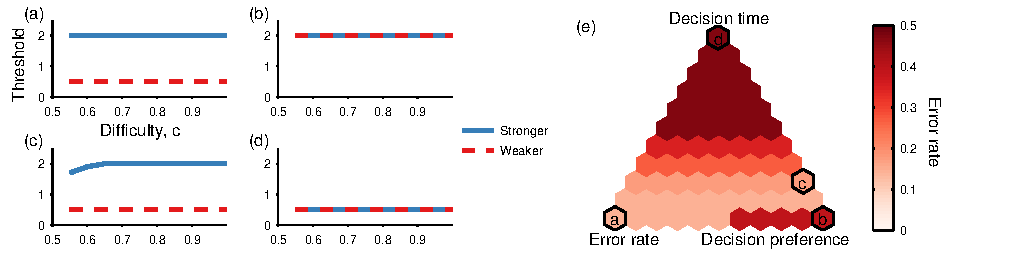
\includegraphics[width=6.83in]{Figure1.pdf}
\caption{\label{nasheq} Nash thresholds depend on the optimization weights. The accuracy of a pair using Nash equilibrium thresholds decreases as the weight given to either decision time or decision preference increases.  In (a)-(d) the lines show the Nash equilibrium thresholds for a pair of animals as a function of the difficulty of the decision ($c$). The optimization weights for each panel are indicated in the simplex with the corresponding letter. In (e) the color indicates the accuracy of a decision made by a pair making a difficult decision ($c=.55$) using Nash equilibrium thresholds, as a function of the optimization weights, $w_1$, $w_2$, $w_3$.  In the lower left corner of the simplex, only error rate matters ($w_1=1$).  In the upper corner, only decision time matters ($w_2=1$).  In the lower right corner, only preference matters ($w_3=1$). Parameters: $w_1=1$, $w_2=0$, $w_3=0$ (a), $w_1=0$, $w_2=0$, $w_3=1$ (b), $w_1=0$, $w_2=0.2$, $w_3=0.8$ (c), $w_1=0$, $w_2=0$, $w_3=1$ (d), $b=1$, $r=1$, $\ell=0.1$ in all panels. }
\end{figure*}

\begin{figure*}[htp]
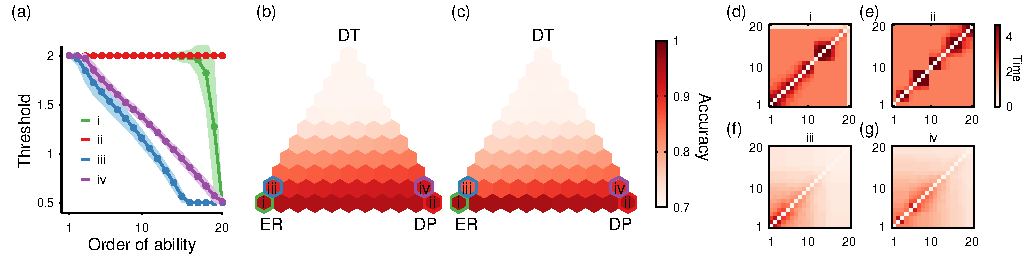
\includegraphics[width=6.83in]{Figure2.pdf}
\caption{\label{groupeq}   The accuracy of a group using Nash thresholds increases as the weight given to decision preference increases as long as there are non-zero waiting costs.  In (a) the points show the average Nash thresholds as a function of position in the group for different optimization weights, where $1$ is the strongest individual and $20$ is the weakest. The shaded region shows the average plus or minus the standard deviation across $1000$ draws.  The optimization weights for each panel are indicated in the simplex with the corresponding letter. The color in the simplex indicates (b) the average accuracy of the whole group and (c) the average accuracy of the decisions made by individuals in the bottom quartile of the group, as a function of the optimization weights, $w_1$, $w_2$, $w_3$.  In the lower left corner of the simplex, only error rate matters ($w_1=1$).  In the upper corner, only decision time matters ($w_2=1$).  In the lower right corner, only preference matters ($w_3=1$).   In (d)-(g) the color indicates the expected time it takes each pair of components to reach a decision in a group using Nash thresholds. Parameters: $w_1=1$, $w_2=0$, $w_3=0$ (i), $w_1=0$, $w_2=0$, $w_3=1$ (ii), $w_1=0.9$, $w_2=0.1$, $w_3=0$ (iii), $w_1=0$, $w_2=0.1$, $w_3=0.9$ (iv), $N=20$, $b=1$, $r=1$, $\ell=0.1$ in all panels. }

\end{figure*}


\begin{figure}[htp]
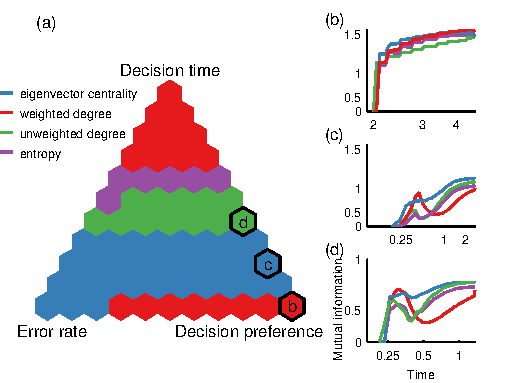
\includegraphics[width=3.4in]{Figure3.pdf}
\caption{\label{bestmetric} The best measure of consensus in the decision network depends on the average error rate and the types of errors being made.  In (a) the color indicates the most informative consensus measure to apply to a network constructed by a group using Nash thresholds, as a function of the optimization weights. In the lower left corner of the simplex, only error rate matters ($w_1=1$).  In the upper corner, only decision time matters ($w_2=1$).  In the lower right corner, only preference matters ($w_3=1$). In (b)-(d) we show how the mutual information of each consensus formalism changes over time as the network forms. The optimization weights for each panel are indicated in the simplex with the corresponding letter. Parameters: $w_1=0$, $w_2=0$, $w_3=1$ (c), $w_1=0$, $w_2=0.2$, $w_3=0.8$ (d), $w_1=0$, $w_2=0.4$, $w_3=0.6$ (e),  $N=20$, $b=1$, $r=1$, $\ell=0.1$ in all panels.}
\end{figure}


\begin{figure}[htp]
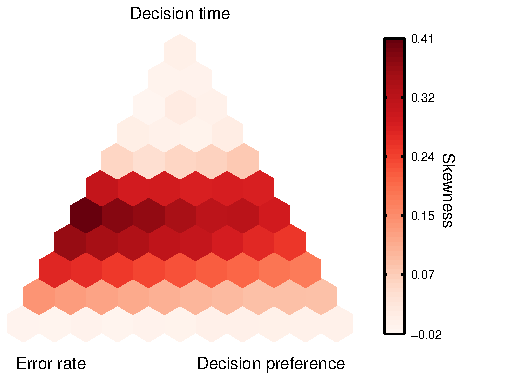
\includegraphics[width=3.4in]{Figure4}
\caption{\label{skewness} The average skewness of the distribution of unweighted in-degree is maximized at intermediate waiting costs. The color indicates the average skewness of the distribution of a group using Nash thresholds, as a function of the optimization weights, $w_1$, $w_2$, $w_3$. In the lower left corner of the simplex, only error rate matters ($w_1=1$).  In the upper corner, only decision time matters ($w_2=1$).  In the lower right corner, only preference matters ($w_3=1$). Parameters: $N=20$, $b=1$, $r=1$, $\ell=0.1$.}
\end{figure}

\begin{table}[h]
\caption{\label{examples}{\bf  Examples of collective computation.} A collective computation can occur when a group of components, each of which gathers information and makes a decision in a noisy environment, produces an output that depends in a complex non-linear way on the individuals' decisions. This phenomenon is found in many biological systems. }
\begin{tabular}{@{\vrule height 10.5pt depth4pt  width0pt}llllll@{}}
System & Information & Component &   Component decision & Collective computation \\
\cline{1-5} 
brain & moving dots& neural population & to stop firing & decision of the brain
\\  social group & fights won or lost & monkey & to emit a subordination signal & power structure
\\  quorum sensing & signaling molecule & bacteria & to produce signaling molecule & production of toxin
\\ flock movement & environment & bird & where to fly and how quickly & flock movement
\\
\hline
\end{tabular}
\end{table}


\begin{table}[ht]
\caption{\label{variables}{ Variables in the model and their interpretations in neural and social systems.} }
\begin{tabular}{@{\vrule height 10.5pt depth4pt  width0pt}llllll@{}}
Variable & Definition & Neural &   Social \\
\cline{1-4} 
$a$  & value &  degree to which the property  & fighting ability
\\ & & a neural population responds to 
\\ & & is present in the environment&
\\ $b$ & change due to new evidence
\\$c$ & strength of input & coherence of dots & probability of stronger animal winning
\\ $\ell$ & leak rate
\\ $r$ & interaction rate 
\\ $T_1,T_2$ & decision thresholds
\\ $w_1$ & error rate weight & reward from being ``correct" & reward from being ``correct"
\\ $w_2$ & decision time weight & penalty for taking a long time & costs of fighting
\\ $w_3$ & probability of preference weight &  & benefit from receiving signal
\\$X_1,X_2$ & decision variables &  firing rates of neural populations & evidence accumulated about relative dominance
\\
\hline
\end{tabular}
\end{table}

%\begin{table}[ht]
%\centering
%\caption{\label{differences}{\bf  Comparison of model in different application.} In its original application to neural systems, the leaky integrator model was reduced to one dimension and the only optimality criteria considered were accuracy and decision time. We study a two-dimensional version of the model and consider the possibility of decision preferences as an additional optimality criterion. This model can be applied to a collection of neural populations in the brain and to a social group of monkeys. Differences between the original neural application and the extended neural and social applications are highlighted in red.}
%\begin{tabular}{@{\vrule height 10.5pt depth4pt  width0pt}llllll@{}}
%  &Original neural & Extended neural & Social \\
%\cline{1-3} \cline{4-4} 
%decision & difference hits a threshold  & ? & \fcolorbox{red}{white}{one var. hits a threshold}
%\\dimensionality & $1$  & $?$ & $2$  
%\\ group size & $2$ &\fcolorbox{red}{white}{$N$}& \fcolorbox{red}{white}{$N$}
%\\ optimality criterion &  reward from being ``right" & reward from being ``right"& reward from being ``right"
%\\ & decision time &decision time & decision time
%\\ & &\fcolorbox{red}{white}{reward from  receiving signal} & \fcolorbox{red}{white}{reward from  receiving signal}
%\\optimization & no &  \fcolorbox{red}{white}{yes} & \fcolorbox{red}{white}{yes} 
%\\ depends on other
%\\  individual's threshold
%\\ \hline
%\end{tabular}
%\end{table}
%
%


\end{document}


